% ------------------------------------------------------------
% Concept note / mini proposal.
%
% Cover pages come from the separate two-page PDF built in
% "Cover Page/src/", included below. Body follows the MSc dissertation
% format, so this file compiles with ordinary pdfLaTeX:
%   tectonic -X compile concept_note.tex
%
% If the cover PDF is missing, build it first:
%   cd "Cover Page/src" && tectonic -X compile cover_concept_note.tex
% ------------------------------------------------------------
\PassOptionsToPackage{final}{graphicx}
\documentclass[12pt,final]{article}

\usepackage{msc_body_style}

\begin{document}

	% =============================================================
	% Cover and title pages (separate document)
	% =============================================================
	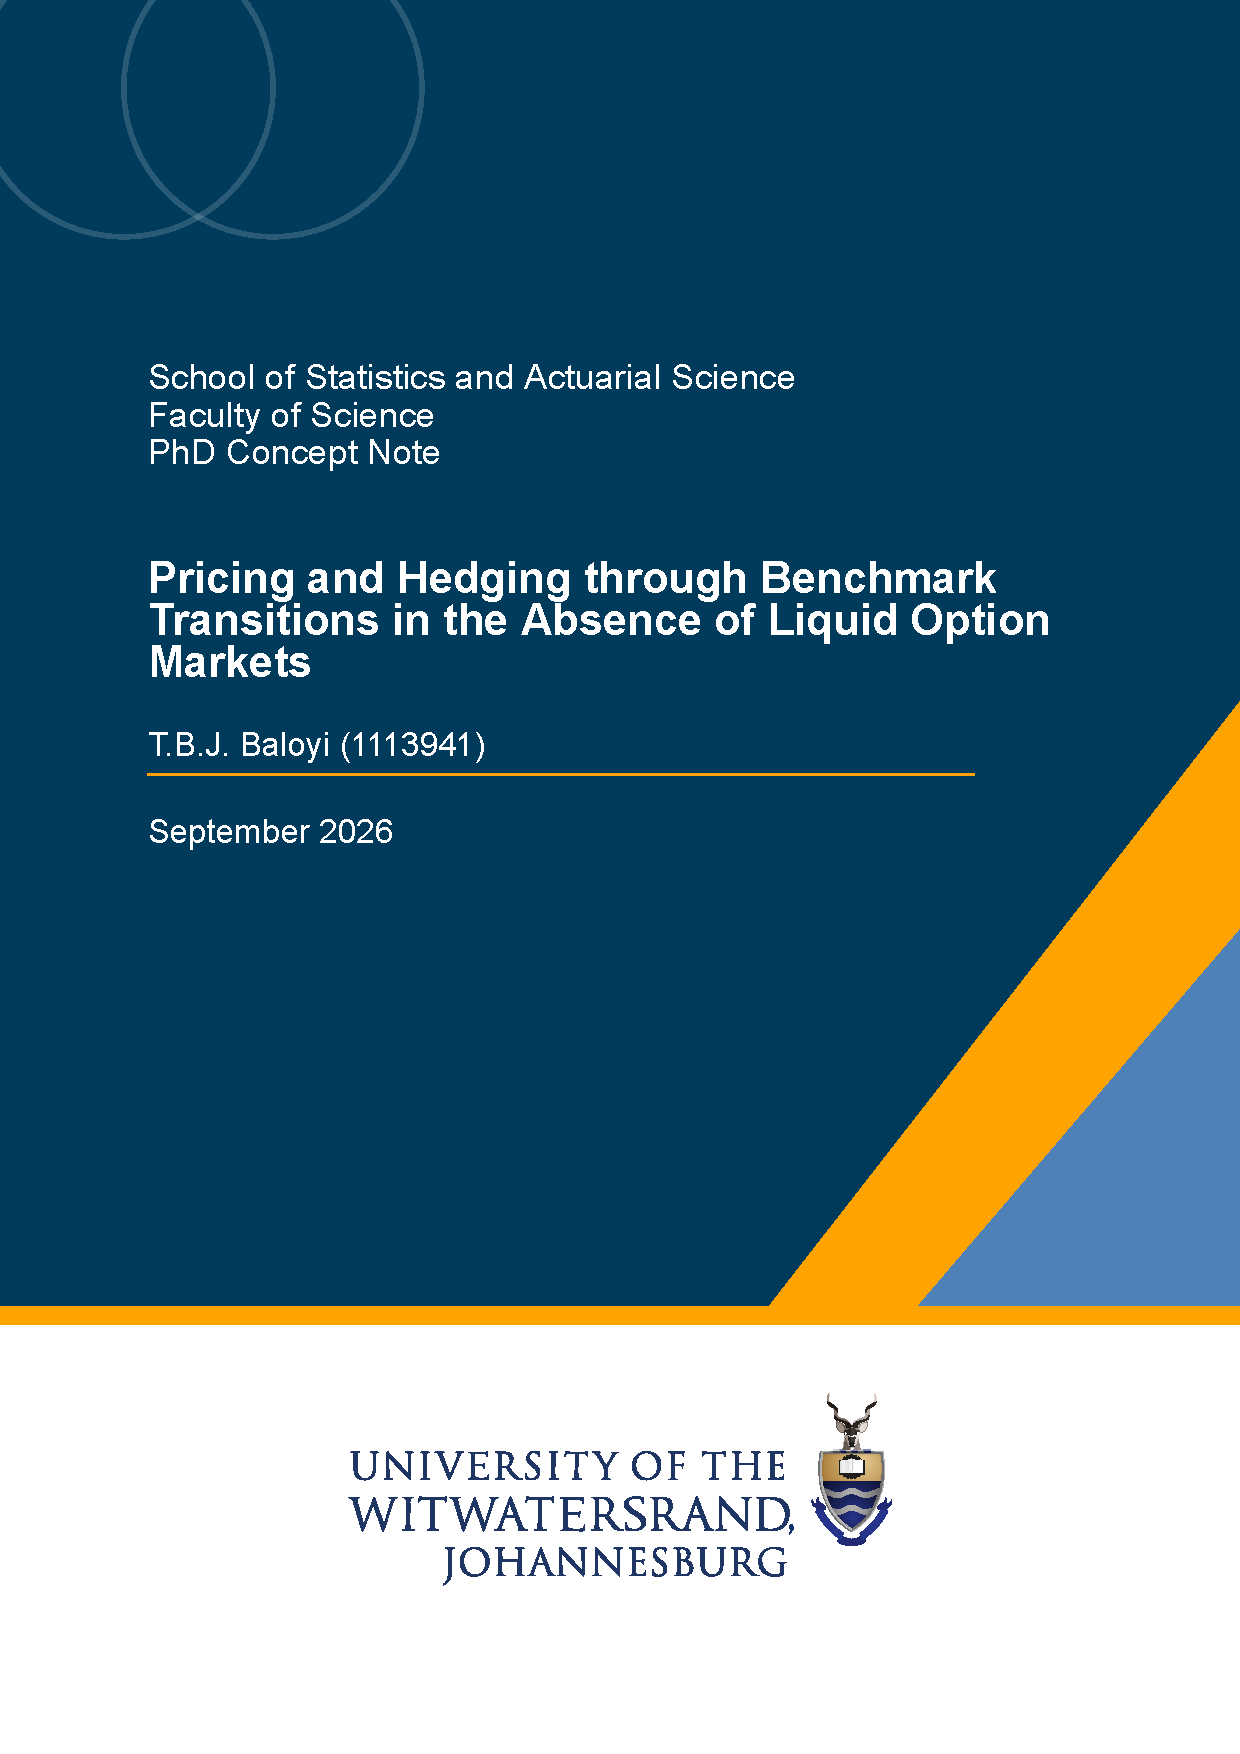
\includepdf[pages=1-2]{Cover Page/src/cover_concept_note.pdf}

	\clearpage
	\pagenumbering{arabic}

	% =============================================================
	\section{Research problem}

	When an interest-rate benchmark is replaced, the contractual cashflows of
	existing derivatives change. A forward-looking term rate, fixed at the start
	of an accrual period, gives way to a rate compounded over that period from
	overnight fixings. This alters both when the underlying is observed and how
	uncertainty accumulates, and it does so for contracts written long before the
	replacement was contemplated.

	The resulting difficulty is informational. A dealer observes a reliable
	market in instruments referencing the legacy benchmark --- curves, swaps,
	basis instruments and legacy options --- while having little or no direct
	evidence about options referencing the successor rate. Those observations
	constrain some features of the transition, but they need not determine the
	full distribution on which an option payoff depends.

	This distinction matters because an option is sensitive to outcomes beyond an
	average rate. Two models can agree on every forward value while assigning
	different probabilities to large rate moves, and a caplet separates them.
	Importing a volatility parameter from the legacy market therefore yields a
	number without establishing that the number follows uniquely from what was
	observed: a fitted model returns a single successor price even when the
	observations are compatible with many.

	A second question concerns trading rather than valuation. Valuation
	uncertainty is the range of model prices compatible with the observations;
	trading risk is the realised profit or loss from holding and hedging the
	liability. A closely calibrated model can still produce large losses when
	trading constraints or changing dynamics bind, and small average hedging
	error says nothing about the upper tail.

	The South African JIBAR--ZARONIA transition supplies the application, with
	South African Reserve Bank conventions \citep{sarb2024conv} governing the
	contractual implementation. Statements about liquidity will be tied to a
	particular instrument, tenor and observation period, established by a data
	audit rather than assumed for the market as a whole.

	% =============================================================
	\section{Research question and sub-questions}

	\begin{quote}
		Under what assumptions can legacy market information determine
		successor-rate option values, and what statistically defensible bounds can
		be placed on the losses from hedging those options through a benchmark
		transition?
	\end{quote}

	\begin{enumerate}
		\item[\textbf{RQ1.}] Which successor valuation functionals are constant across the models compatible with legacy option quotes and curve or basis observations?
		\item[\textbf{RQ2.}] Which additional observations or restrictions restore identification, and how stable is that conclusion under quote noise?
		\item[\textbf{RQ3.}] Under what dependence and distribution-shift assumptions does a calibrated loss threshold retain a finite-sample guarantee?
		\item[\textbf{RQ4.}] Are the resulting price ranges and risk bounds informative for a realistic hedge once costs and data limitations are included?
	\end{enumerate}

	% =============================================================
	\section{Aim and objectives}

	\textbf{Aim.} To develop and evaluate a framework for identifying
	successor-rate option valuations and quantifying residual hedging risk under
	limited option-market information.

	\begin{enumerate}
		\item Specify a transition model, contractual conventions and observable market information, keeping risk-neutral pricing assumptions separate from historical estimation.
		\item Establish identification or non-identification results for a restricted model class, and determine the resulting valuation ranges and approximation errors.
		\item Construct implementable hedges from available instruments and derive finite-sample loss guarantees under explicit assumptions.
		\item Evaluate pricing uncertainty, hedge performance and threshold informativeness in simulation and in an empirical application.
	\end{enumerate}

	% =============================================================
	\section{Scope}

	The initial product scope is caplets, with compounding, observation shift and
	payment conventions stated explicitly rather than inferred from a
	similar-looking formula. The model is a small factor system, and the hedge
	set is liquid swaps and cash instruments, restricted to instruments shown to
	be tradeable on the relevant date. A successor option is not used as a
	hedging instrument merely because it would complete the market.

	Swaptions, large portfolios, jump extensions, multi-tenor consistency,
	learned hedging policies and rough-path methods are extensions, each taken up
	only where it answers a stated research question. The collateral and funding
	structure is simplified, and that simplification is stated.

	The application is the JIBAR--ZARONIA transition. A retrospective study in a
	currency where successor options did trade offers a further validation route,
	subject to licensed and comparable data.

	% =============================================================
	\section{Literature and research gap}

	\citet{brigo2006} supply the pricing architecture, \citet{lyashenko2019}
	develop a forward-market treatment of backward-looking rates, and
	\citet{willems2020} studies SABR smiles for risk-free-rate caplets. These set
	the modelling framework, but none establishes that successor smiles are
	identified from a given set of legacy observations.

	Local work supplies method and context: \citet{konaite2024} on the forward
	market model, \citet{menziwa2023} on pricing, calibration and hedging under
	the LIBOR model, \citet{robbertze2021} on neural-network volatility modelling
	and \citet{stangroom2023} on deep hedging. \citet{mavuso2014} studies
	mean--variance hedging with a dynamically traded liquid asset and a static
	position in an illiquid one, which makes trading permissions part of the
	mathematical problem. \citet{feng2018} separate calibration from
	recalibration model risk. \citet{alfeus2026} models JIBAR--ZARONIA spread
	dynamics around scheduled events; that is historical spread modelling, and is
	distinct from identifying a risk-neutral option valuation.

	The statistical component builds on conformal prediction. \citet{vovk2012}
	treats conditional validity, \citet{barber2023} departures from
	exchangeability, and \citet{oliveira2024} split conformal prediction for
	non-exchangeable data; \citet{barber2026} and \citet{ramos2026} are closest
	to the dependence and calibration-conditional questions at issue.

	The gap lies between these two literatures: a rigorously characterised set of
	transition models on one side, and a finite-sample analysis of the hedging
	losses those models imply on the other, under stated dependence and
	distributional change. Connecting them is the object of this research.

	% =============================================================
	\section{Approach}

	\subsection{Model and observations}

	The work begins with a low-dimensional Markov model in an overnight-rate
	factor and a spread factor, with a stated correlation, under an explicit
	pricing measure. A two-factor Gaussian diffusion serves as the analytical
	benchmark: it admits explicit covariance calculations and tractable
	simulation, and its restrictions, including the possibility of negative
	rates, are recorded. The observation map from model to traded instrument
	prices is specified so that it prices actual cashflows before any
	identification claim is made.

	\subsection{Identification}

	Let $O$ denote the observations available at a valuation date and
	$\Lambda(\theta)$ the model-implied observation vector. The compatible set is
	\begin{equation}
		\Theta(O) = \{\theta \in \Theta : \Lambda(\theta) \text{ is compatible with } O\},
	\end{equation}
	with compatibility defined by quote tolerances, preferably observed bid--ask
	ranges. A target valuation is identified when it is constant on $\Theta(O)$;
	otherwise the attainable range runs between
	$V_{-} = \inf_{\theta \in \Theta(O)} V_{\theta}$ and
	$V_{+} = \sup_{\theta \in \Theta(O)} V_{\theta}$. These are identification
	ranges rather than confidence intervals. Non-identification is established
	constructively, by exhibiting two admissible models that share the full
	observation map and disagree on the target; identification requires
	constancy across the entire compatible set.

	A one-period calculation shows the mechanism. Let a successor shock
	$X = \sigma Z_1$ and a basis shock
	$B = \eta(\rho Z_1 + \sqrt{1-\rho^2}\,Z_2)$ combine into a legacy shock
	$Y = X + B$. If an idealised legacy surface identifies $Y$ as standard
	normal, that is one equation in three covariance parameters. With $\rho = 0$,
	both $\sigma = \eta = 1/\sqrt{2}$ and $\sigma = 1/2$, $\eta = \sqrt{3}/2$
	reproduce it exactly, so every payoff depending only on $Y$ is priced
	identically. A zero-strike call on $X$ is worth $\sigma/\sqrt{2\pi}$:
	approximately $0.2821$ in the first case and $0.1995$ in the second.
	Agreement on the entire legacy distribution leaves the successor payoff
	undetermined. The thesis establishes whether this variation survives once
	curves, basis instruments, multiple maturities and any available options
	enter the observation map.

	\subsection{Hedging}

	Discounted terminal wealth comprises initial capital, cumulative trading
	gains and transaction costs; signed hedging loss is the discounted liability
	less that wealth. A sensitivity hedge and a mean--variance hedge provide the
	initial comparisons, with admissibility, financing, rebalancing and costs
	fixed before evaluation. Hedges are compared across compatible pricing models
	on common evaluation scenarios.

	\subsection{Finite-sample guarantees}

	The statistical object is an upper threshold for a future hedging loss. The
	baseline is split conformal calibration for a hedge frozen before
	calibration, whose order-statistic threshold carries an exact finite-sample
	marginal guarantee under exchangeability, with a Beta law describing realised
	calibration-conditional coverage in the continuous independent case. The
	extension separates scores by a declared gap and uses coupling under a stated
	mixing condition to control dependence, together with a distance between
	calibration and test loss distributions to control shift, giving a guarantee
	of the form
	\begin{equation}
		\Pr\{L_{\mathrm{new}} \leq q\} \geq 1 - \alpha - \varepsilon_{\mathrm{dep}} - \varepsilon_{\mathrm{shift}} - \varepsilon_{\mathrm{est}}.
	\end{equation}
	Since neither unrestricted shift nor unrestricted dependence can be bounded
	from a short historical sample, oracle simulation, sensitivity analysis under
	declared budgets and estimated bounds are reported separately, and the
	regimes in which the bound becomes uninformative are identified.

	% =============================================================
	\section{Validation and data}

	Three settings are used. \textbf{Controlled simulation} generates data from
	specified transition models with known targets, varying basis volatility,
	dependence, maturity, strike, observation noise, costs and regime changes,
	and including deliberately misspecified models. \textbf{Retrospective
	validation} withholds successor option quotes while fitting to permitted
	legacy and curve information, revealing them only for evaluation; a
	historical LIBOR--SOFR dataset is the candidate, subject to availability and
	comparability. \textbf{The South African application} proceeds on the
	instruments and dates the data audit supports, reporting compatible valuation
	ranges, scenario sensitivity and observable hedge outcomes.

	Training, method selection, calibration and final evaluation are separated
	chronologically, with gaps where the dependence argument requires them, so
	that withheld data cannot enter calibration through model selection.

	Data access is the principal feasibility consideration. Where licensed option
	or hedge data cannot be obtained, the empirical design reduces to what the
	available observations support, with simulation carrying the controlled
	validation.

	% =============================================================
	\section{Contribution}

	The contribution has two linked parts: an identification analysis for a
	restricted benchmark-transition model and observation set, determining which
	successor valuations the legacy market fixes and how wide the remaining range
	is; and a finite-sample analysis of loss thresholds for implementable hedges
	under specified dependence and distributional change. Together these say what
	a converted option book can be valued at on the evidence available, and what
	can be guaranteed about the losses from hedging it.

	% =============================================================
	\section{Indicative timeline}

	\begin{table}[H]
		\centering
		\caption{Indicative full-time schedule.}
		\label{tab:timeline}
		\begin{tabular}{@{}ll@{}}
			\toprule
			\textbf{Months} & \textbf{Work} \\
			\midrule
			1--6   & Foundations, literature review and data audit \\
			7--14  & Transition model and identification \\
			15--22 & Hedging and statistical analysis \\
			23--29 & Simulation and empirical evaluation \\
			30--36 & Synthesis, revision and examination preparation \\
			\bottomrule
		\end{tabular}
	\end{table}

	Month 6 is the first review point, confirming data access, the model class
	and the direction of the identification results before implementation is
	expanded.

	% =============================================================
	\newpage
	\nocite{sarb2024conv}
	\bibliographystyle{plainnat}
	\bibliography{../../References}
	\addcontentsline{toc}{section}{References}

\end{document}
